\section{Waves}
\footnotetext{Notes based on 3blue1brown/minutephysics \url{https://www.youtube.com/watch?v=MzRCDLre1b4}}

The late 1800s understanding of light (marked by Maxwell's Equations) was that it consists of waves
in the electromagnetic field.

The electromagnetic field comprises an \defn{electric field} and a \defn{magnetic field}. These are
both vector fields: i.e. they consist of a vector-valued quantity at every location $x$ in
3-dimensional space. The field changes over time, so can be written as a vector-valued function of
$(x, t)$.

{\bf Electric field: $\vec E(x, t)$)} Suppose a charged particle is at location $x$. Then there is a
force on the particle dependent on the field value $\vec E(x, t)$ and the charge of the particle.

{\bf Magnetic field: $\vec B(x, t)$} Suppose a particle with charge $q$ is moving with velocity
$\vec v$ in a magnetic field $\vec B(x, t)$. Then there is a force on the particle equal to
$q\vec v \times \vec B(x, t)$\footnote{$\times$ is a cross product of vector-valued quantities, so
  this means that the direction of the force is perpendicular to both the velocity direction and the
  field direction at that location, and that the magnitude of the force is equal to the product of
  their magnitudes and the charge $q$.}.

Maxwell's equations describe how these two vector fields interact. \footnotetext{In the video, it is
  mentioned that a region of circular flow in one of the fields causes the other field within that
  region to point perpendicular to the plane of the loop.} The end result is that in an
electromagnetic wave, the electric and magnetic fields oscillate, perpendicular to each other, and
perpendicular to the direction of propagation.

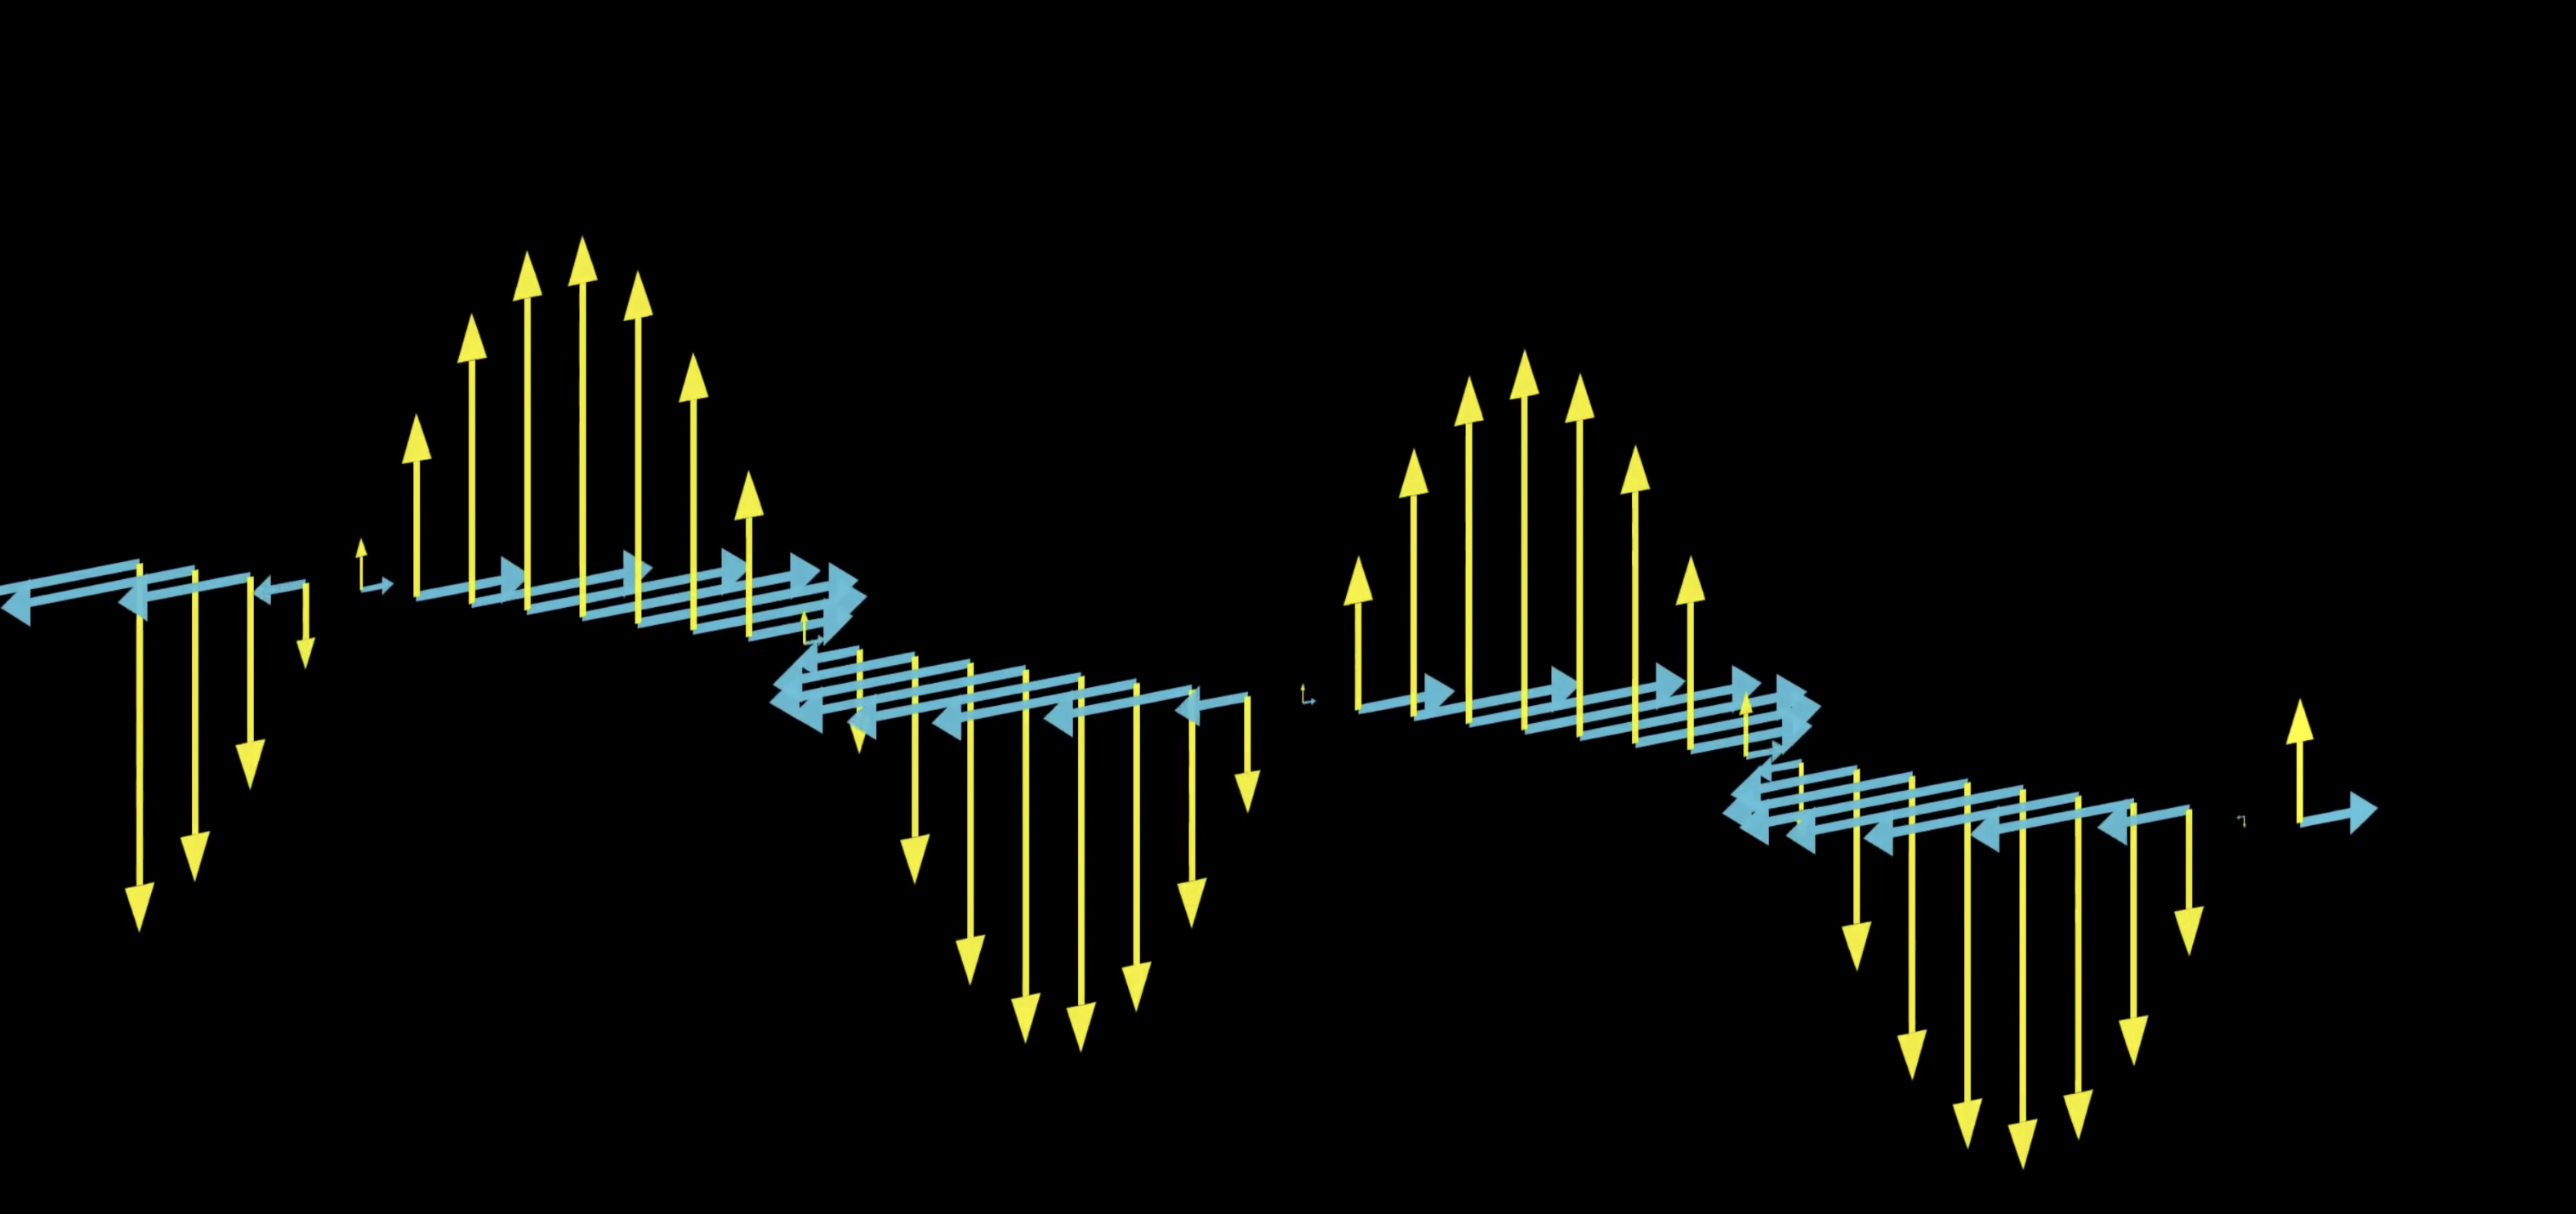
\includegraphics[width=250pt]{img/quantum-waves-1.png}

In the above screenshot, the longitudinal axis of the wave represents space $x$. Time $t$ is
depicted via animation: the vector component of the blue field, at a single spatial location $x$,
grows and shrinks and changes direction over time.

We now view the wave head-on, focusing on a slice at a single spatial location, moving in the plane
perpendicular to the direction of propagation of the wave:

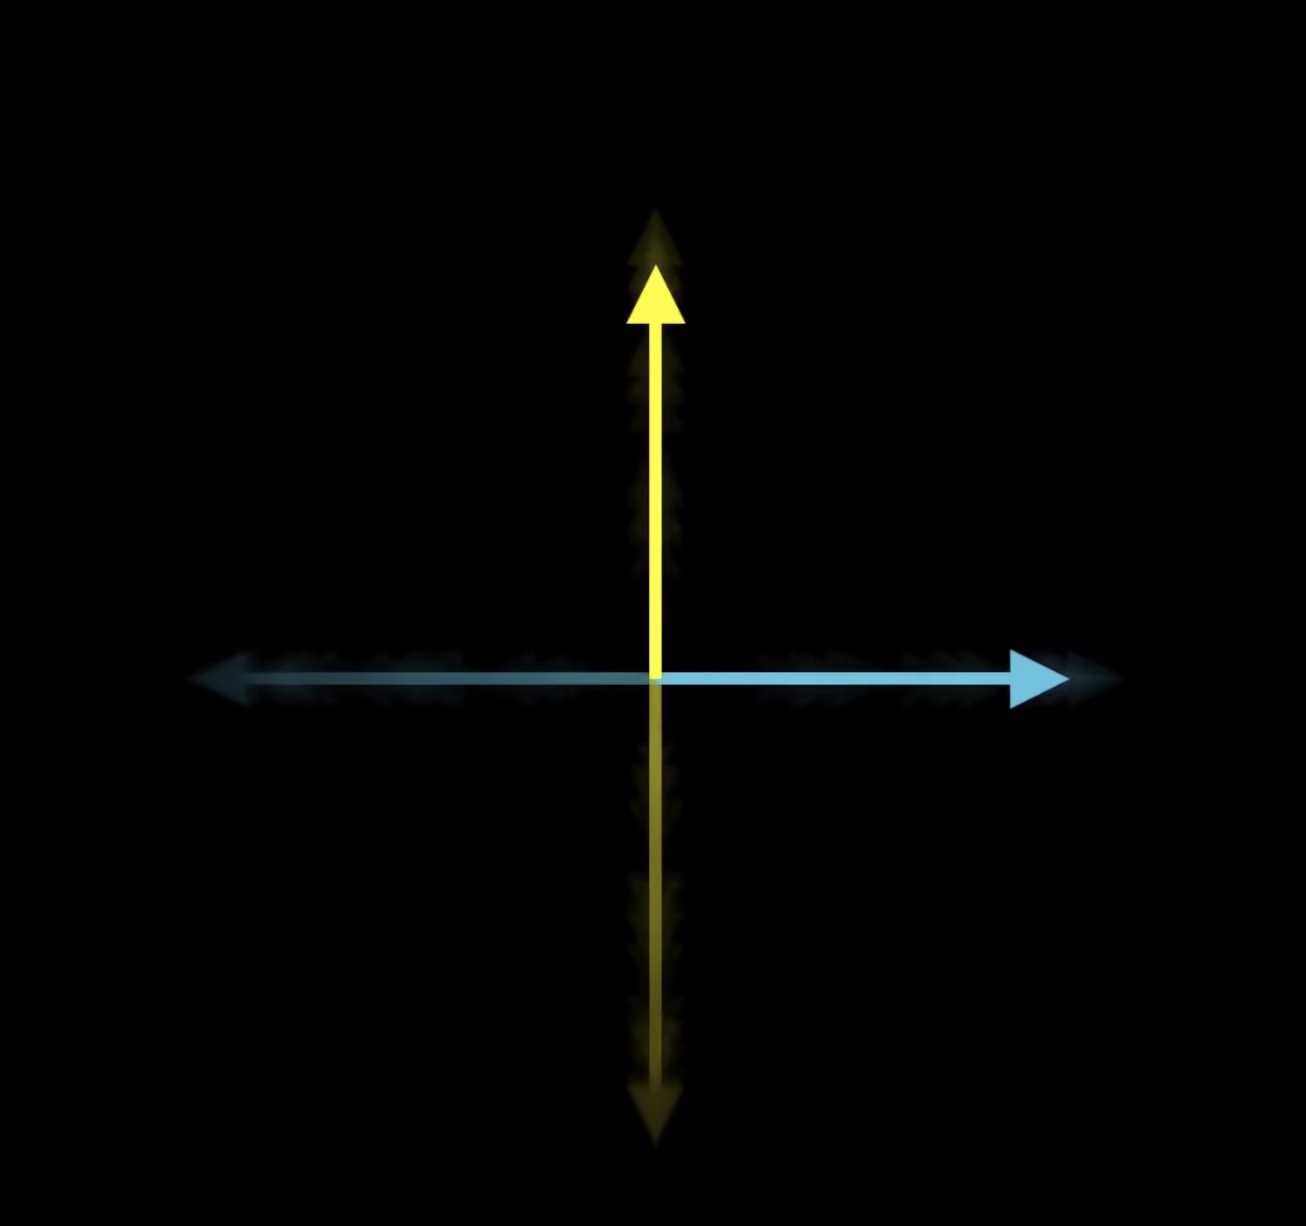
\includegraphics[width=100pt]{img/quantum-waves-2.png}

And we focus on the dynamics of the blue vector component:

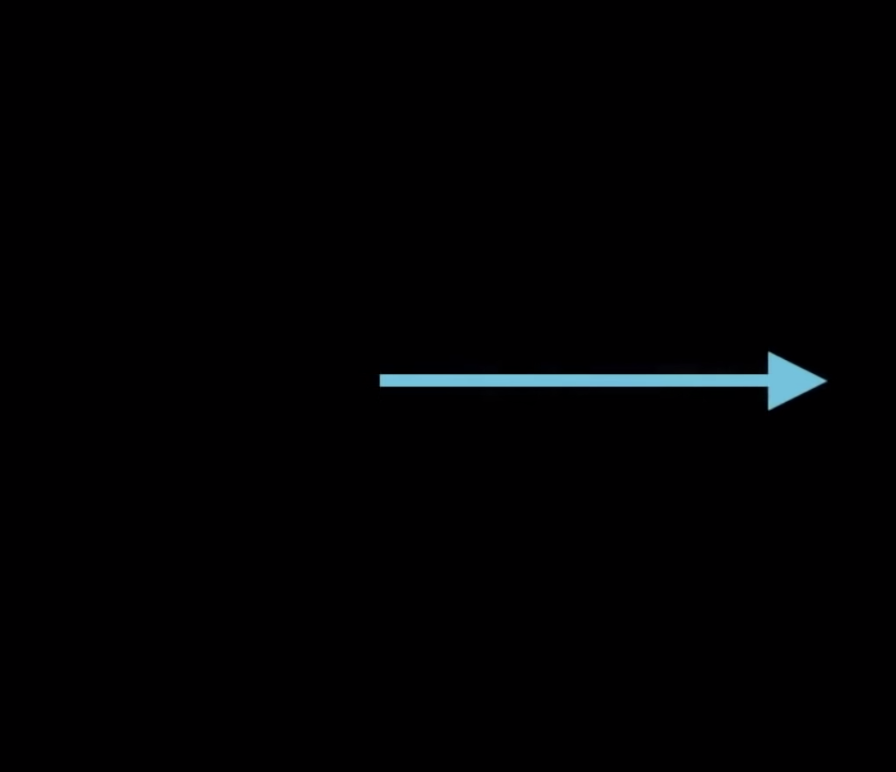
\includegraphics[width=100pt]{img/quantum-waves-3.png}

We use a column vector to represent its position in the left-right and up-down directions, as a
function of time. Since it is moving horizontally, its up-down value is constant at zero, and its
left-right dynamics can be described by a cosine function of time (with time scaled by $2\pi$ so
that one cosine oscillation is completed in one unit of time):
\begin{align*}
  \vecMM{\cos(2\pi t)}{0}.
\end{align*}
We add a parameter $f$ controlling its frequency of oscillation, and a parameter $A$ controlling its
amplitude:
\begin{align*}
  \vecMM{A\cos(2\pi ft)}{0}.
\end{align*}
Critically, we also include a parameter $\phi$ controlling the phase of this oscillation, i.e. when
in time its low/high points occur:
\begin{align*}
  \vecMM{A\cos(2\pi ft + \phi)}{0}.
\end{align*}

\subsection*{Questions}
\begin{enumerate}
\item What exactly does ``wave propagation'' mean?
\item In principle, presumably, vectors in the electric and magnetic vector fields can point in any
  direction in 3D space. What are the constraints on this when we are considering a ``wave''?
\end{enumerate}

% \newpage
% See \ref{real-and-complex-vector-spaces}
% \section{Adjoint, Unitary matrices, etc}\label{adjoint-and-unitary-matrices}
% The \defn{conjugate transpose} or \defn{adjoint} or \defn{Hermitian conjugate} of a matrix is formed
% by taking the transpose, and then replacing each element with its complex conjugate:
% \begin{align*}
%   U^\dag = \bar{U^T}.
% \end{align*}
% It is also written as $U^*$ or $U^H$.

% A matrix $U$ is \defn{unitary} if $U^\dag U = I$.

% \newpage
% \section{The qubit}
% \footnotetext{Notes based on Michael Nielsen - Quantum Computing for the Very Curious \url{https://quantum.country/qcvc}}

% The state of a qubit is a unit vector in a two-dimensional complex vector space. The basis vectors
% are written $\ket{0}$ and $\ket{1}$, so a qubit is
% \begin{align*}
%   \alpha\ket{0} + \beta\ket{1}
% \end{align*}
% where $\alpha, \beta \in \C$ with $|\alpha|^2 + |\beta|^2 = 1$.

% What does the normalization constraint $|\alpha|^2 + |\beta|^2 = 1$ mean geometrically? If
% $\alpha = 0$ then $\beta$ lies on the unit circle, and vice versa.

% How can we visualize the possible values of a qubit?

% Perhaps like this? This diagram illustrates that we pick two complex numbers, $\alpha$ and $\beta$,
% and that they satisfy $|\alpha|^2 + |\beta^2| = 1$.\\
% 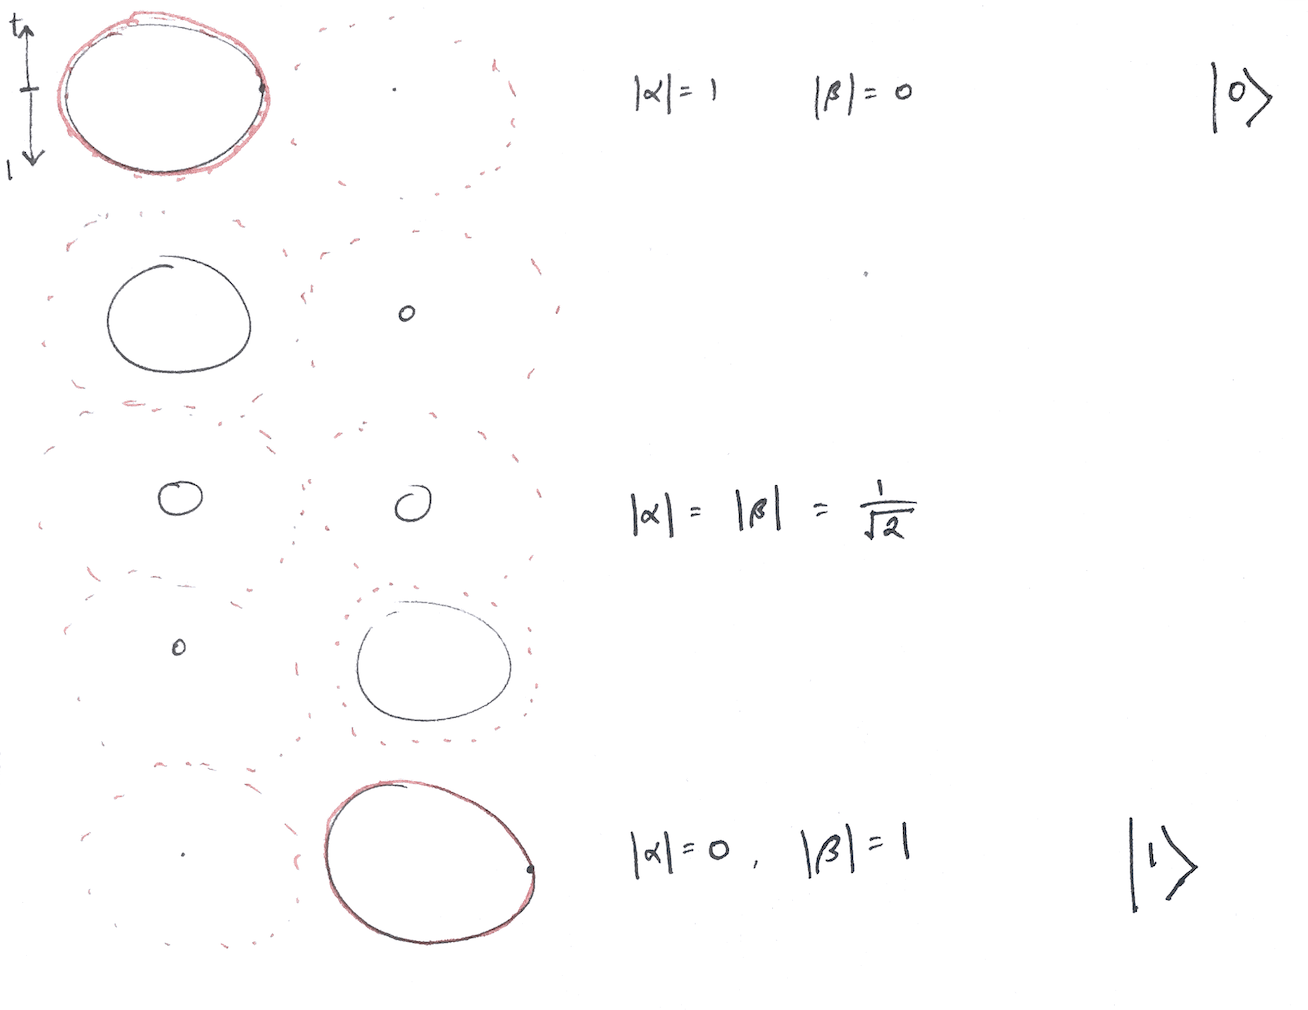
\includegraphics[width=200pt]{img/quantum-qubit-2.png}

% Or like this? Visualize $(|\alpha|, |\beta|)$ as a point on the unit circle and place a clockface at
% that point with two hands, representing the argument
% of $\alpha$ and $\beta$.\\
% 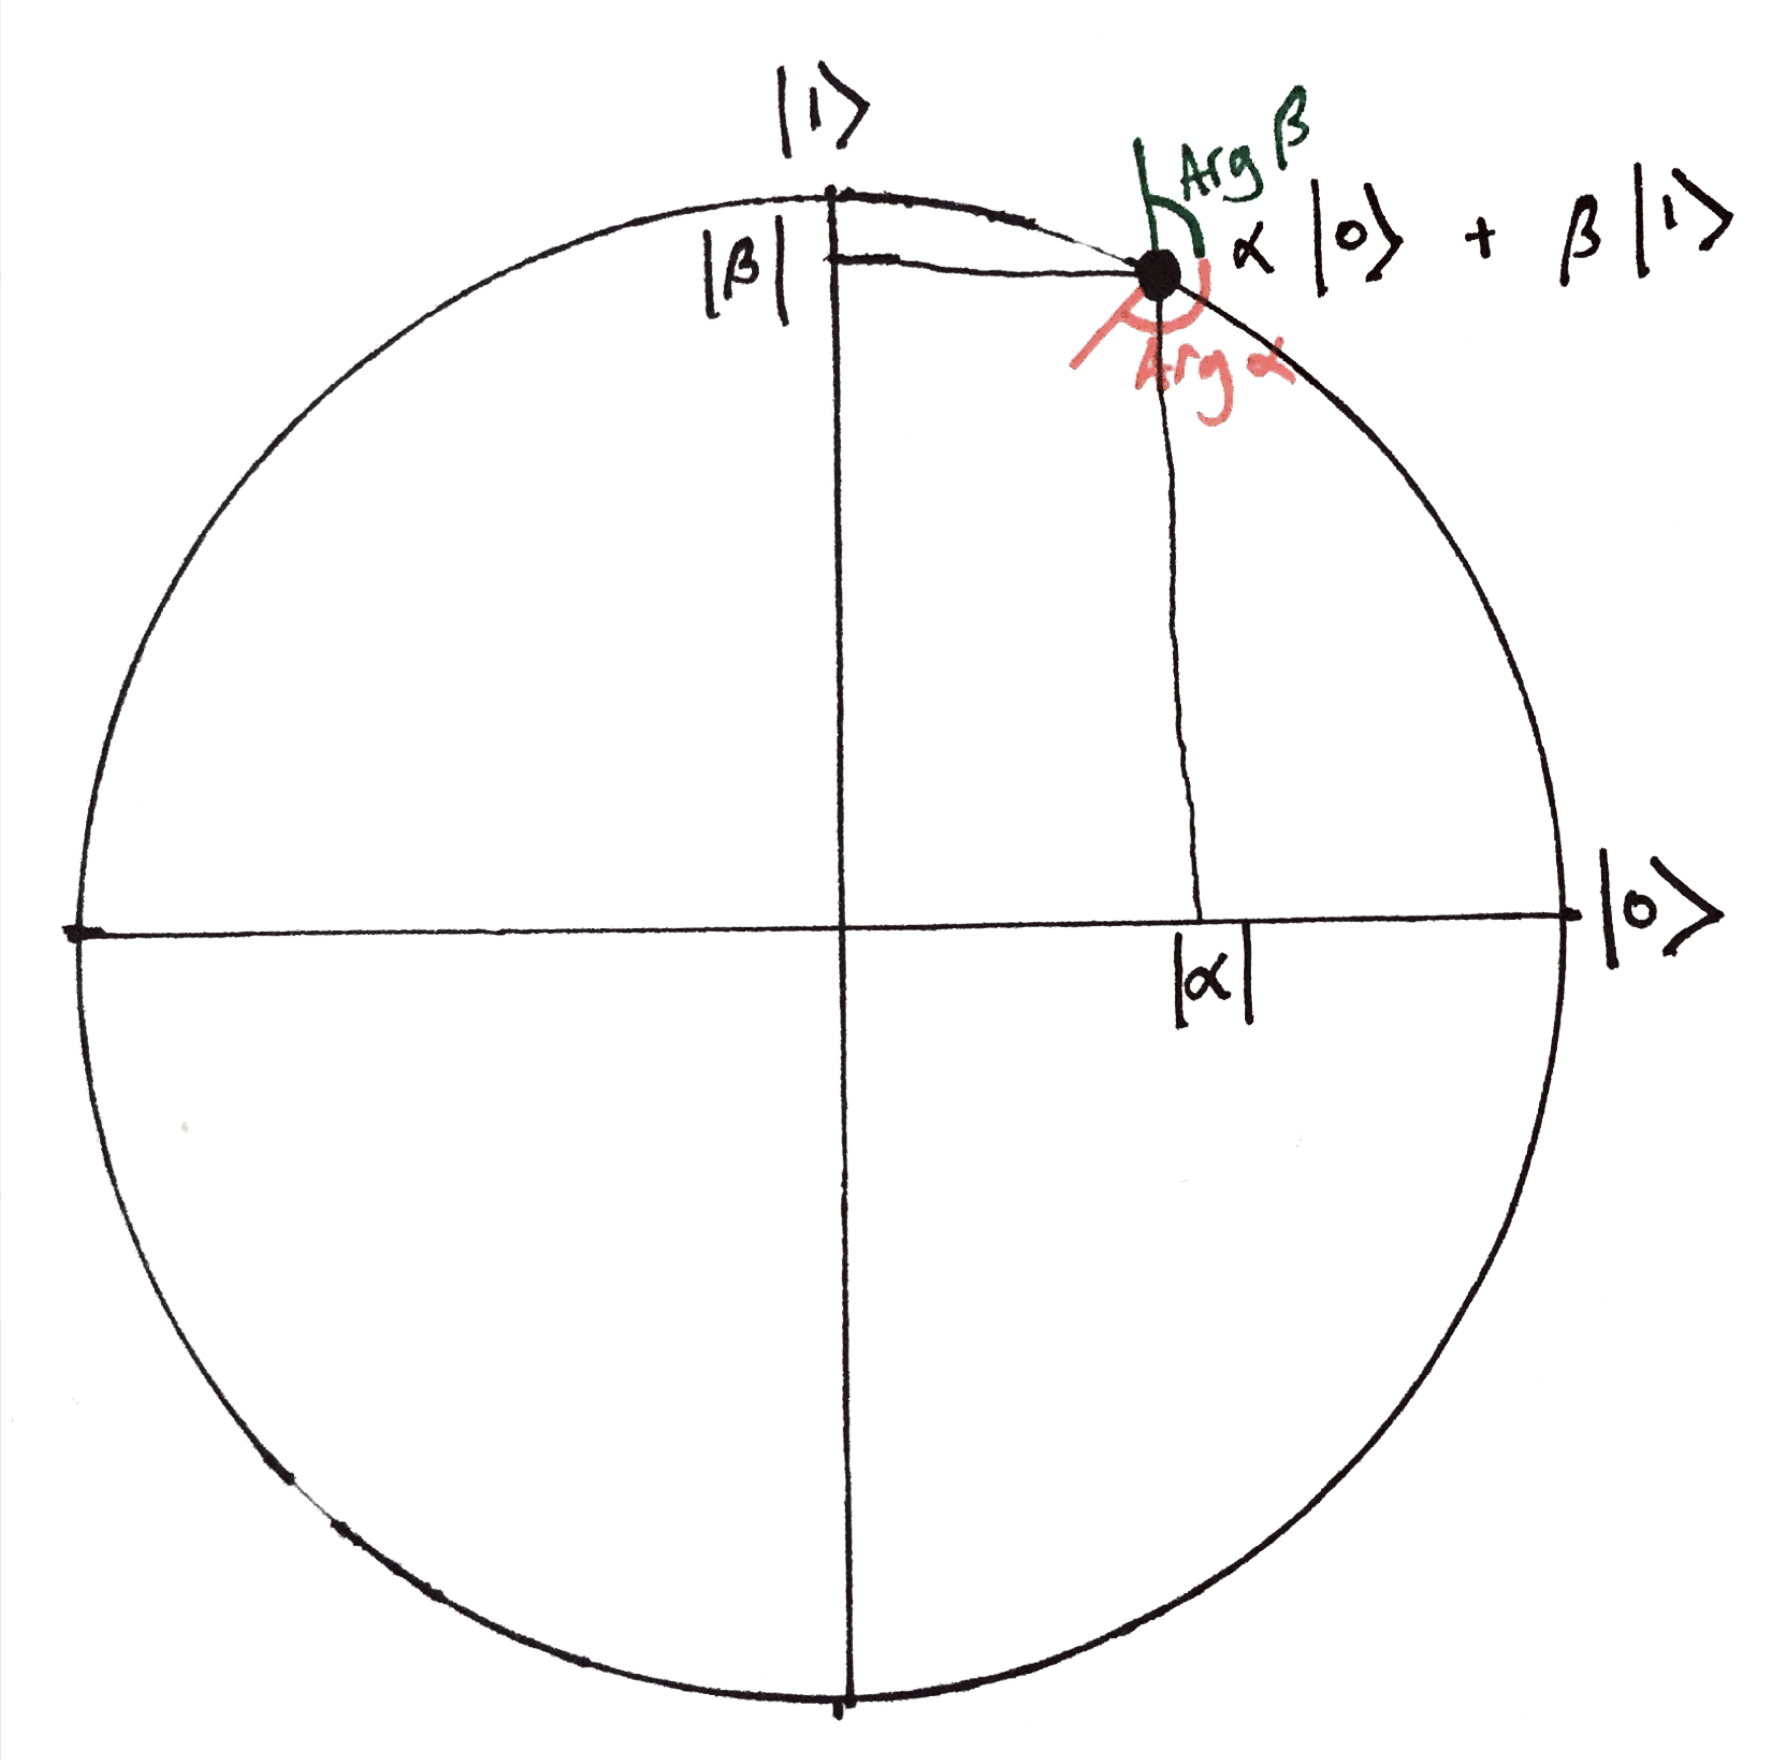
\includegraphics[width=200pt]{img/quantum-qubit.png}


% \newpage


% \newpage
% \section{Quantum logic gates}

% These are linear operators that act on a qubit state to produce a new qubit state. Therefore they
% are $2 \times 2$ complex matrices. Since they unitary
% \begin{enumerate}
% \item {\bf Not}
%   \begin{align*}
%     X = \matMMxNN{0}{1}
%     {1}{0}
%   \end{align*}
% \item {\bf Hadamard}
%   \begin{align*}
%     H = \frac{1}{\sqrt{2}}\matMMxNN{1}{1}
%     {1}{-1}
%   \end{align*}
% \item {\bf $Y$}
%   \begin{align*}
%     Y = \matMMxNN{0}{-i}
%                  {i}{0}
%   \end{align*}
% \item {\bf $Z$}
%   \begin{align*}
%     Z = \matMMxNN{1}{0}
%                  {0}{-1}
%   \end{align*}
% \end{enumerate}

% The not gate essentially swaps the two dimensions: the coefficient of $\ket{0}$ becomes the
% coefficient of $\ket{1}$ and vice versa. So e.g.
% \begin{align*}
%   X\ket{0} &= \ket{1}\\
%   X\ket{1} &= \ket{0},
% \end{align*}
% and by linearity
% \begin{align*}
%   X \(\alpha \ket{0} + \beta \ket{1}\) = \beta \ket{0} + \alpha \ket{1}
% \end{align*}

% Since they are real and symmetric, we have $X^\dag = X$ and $H^\dag = H$. And since
% \begin{align*}
%   X^2 &= I\\
%   H^2 &= \frac{1}{2}\matMMxNN{2}{0}
%         {0}{2} = I,
% \end{align*}\
% we have that $X$ and $H$ are unitary.


% % \begin{align*}
% %   H \ket{0} &= \frac{\ket{0}}{\sqrt{2}} + \frac{\ket{1}}{\sqrt{2}}\\
% %   H \ket{1} &= \frac{\ket{0}}{\sqrt{2}} - \frac{\ket{1}}{\sqrt{2}}
% % \end{align*}
